\documentclass[pra,12pt]{revtex4}
\usepackage{amsmath}
\usepackage{amssymb}
\usepackage{graphicx}
\usepackage{color}
\usepackage{mathrsfs}
\usepackage[pdfborder={0 0 0},colorlinks=true,linkcolor=blue]{hyperref}

\def\ket#1{\left|#1\right\rangle}
\def\bra#1{\left\langle#1\right|}
\def\braket#1{\left\langle#1\right\rangle}

\setlength{\parindent}{0pt}

\renewcommand{\baselinestretch}{1.0}
\setlength{\parskip}{0.07in}

\begin{document}

\begin{center}
{\Large \textbf{Chapter 1: Resonances}}
\end{center}

\section{Bound states and free states}

One of the most interesting features of wavefunctions in infinite
space is that they come in two distinct types: (i) \textbf{bound
  states}, which are localized to one region, and (ii) \textbf{free
  states}, which extend over the entire space.  Both types can
co-exist in a single system.

The \textbf{1D finite square well} is a simple model which exhibits
both bound states and free states.  Consider the Hamiltonian
$$\hat{H} = \frac{\hat{p}^2}{2m} - U \,\Theta(a -|\hat{x}|),$$
where $\hat{x}$ and $\hat{p}$ are the 1D position and momentum
operators, $m$ is the particle mass, $U$ and $a$ are positive real
parameters governing the potential function, and $\Theta(\cdots)$
denotes the Heaviside step function (1 if the input is positive, and 0
otherwise).  As shown below, the potential forms a well of depth $U$
and width $2a$.  Outside the well, the potential is zero.

\begin{figure}[h]
  \centering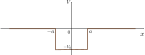
\includegraphics[width=0.7\textwidth]{squarewell}
\end{figure}

We wish to solve the time-independent Schr\"odinger equation for this
Hamiltonian.  A common numerical method, known as the \textbf{transfer
  matrix method}, can be used to generate solutions for this potential
and other similar 1D potentials.  This method is described in Appendix
B.  In this section, we will bypass the details of the calculation,
and instead zoom in on certain key aspects.

The first thing to note is that when solving the Schr\"odinger wave
equation, it's necessary to specify the boundary conditions at
infinity.  This choice determines whether we get a bound state or free
state.  The wavefunction of a bound state diminishes exponentially as
$x \rightarrow \pm\infty$; thus, in the exterior region (i.e., $x <
-a$ or $x > a$), it satisfies
$$-\frac{\hbar^2}{2m}\,\frac{d^2\psi}{dx^2} = E \psi(x),$$
subject to the boundary conditions
$$\psi(x) \overset{x\rightarrow\pm\infty}{\sim} e^{\mp\kappa x}, \;\;\;\mathrm{Re}(\kappa) > 0.$$
The bound state solutions in the exterior region therefore take the
form
$$\psi(x) = c_\pm\, e^{\mp\kappa x}, \;\;\mathrm{where}\;\, -\frac{\hbar^2\kappa^2}{2m} = E, \;\; c_\pm \in \mathbb{C}.$$
Since $E$ is real, it follows that $\kappa$ is real, and hence $E <
0$.  Moreover, the variational principle implies that $E \ge -U$.
Hence, bound state energies are restricted to the range $-U \le E <
0$.  We can also show that the bound state energies are
\textit{discrete}: the energy spacing decreases with $a$, but so long
as $a$ is finite, the spacing is non-vanishing.  Another related
fact is that the wavefunction for a bound state can always be
normalized:
$$\int_{-\infty}^\infty |\psi(x)|^2\, dx\; =\; 1.$$
The normalization integral will not diverge, as $|\psi(x)|^2$ vanishes
exponentially as $x \rightarrow \pm \infty$.

For a free state, the situation is quite different.  In this case, the
wavefunction does not vanish exponentially at infinity, but instead
takes the form
$$\psi(x) = \begin{cases} \alpha_-\, e^{ik x} + \beta_-\, e^{-ik x}, & \;\;\;x < -a\\ (\mathrm{something}) , & -a < x < a\\ \alpha_+\, e^{ik x} + \beta_+\, e^{-ik x} , & \;\;\,x > a.\end{cases}$$
Outside the potential well, $\psi(x)$ consists of a superposition of
left-moving and right-moving plane waves, with wavenumber $k$.  The
coefficients $\alpha_\pm$ and $\beta_\pm$ are not independent
quantities, but are linked by a linear relation (see Appendix B).  In
order to satisfy Schr\"odinger's equation, $k$ must satisfy
$$\frac{\hbar^2k^2}{2m} = E,$$
which means that free states occur only for energies $E \ge 0$.  In
fact, the solutions form a continuum, meaning we can find free states
for \textit{every} $E \ge 0$.  Since $|\psi(x)|^2$ does not diminish
exponentially at infinity, the integral $\int_{-\infty}^\infty
|\psi(x)|^2\, dx$ is divergent.  Hence, the wavefunction has no finite
normalization.

The following figure shows numerically-obtained results for a square
well with $U = 30$ and $a=1$ (in units where $\hbar = m =1$).  The
energy spectrum is shown on the left side.  There exist five bound
states; their plots of $|\psi|^2$ versus $x$ are shown on the right
side.  These results were computed using the transfer matrix code
described in Appendix B.

\begin{figure}[h]
  \centering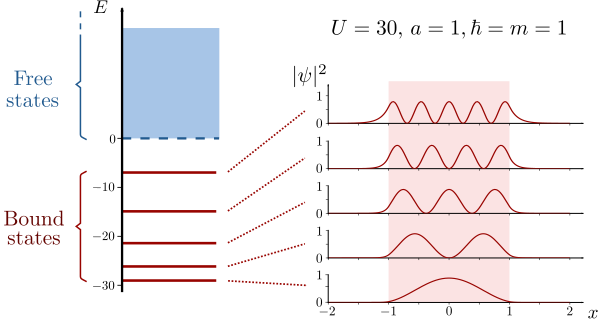
\includegraphics[width=0.81\textwidth]{boundvsextended}
\end{figure}

Many of the lessons drawn from this square well model can be
generalized to more complicated potential wells.  (Also, in cases
where the potential at infinity is $V_{\textrm{ext}}$ rather than
zero, free states occur for $E \ge V_{\textrm{ext}}$ and bound states
occur for $\textrm{min}(V) < E < V_{\textrm{ext}}$.)

There is, however, a proviso to bear in mind.  If we vary the
potential, the number of bound states can change: i.e., bound state
solutions can either appear or disappear.  A numerical example is
given below, showing the bound state energies for the square well
model with fixed $a = 1$, as we vary the potential minimum $-U$:

\begin{figure}[h]
  \centering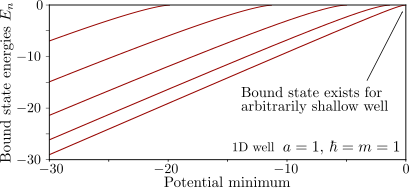
\includegraphics[width=0.65\textwidth]{boundstate1d}
\end{figure}

For $U = 30$, there are five bound states, but these disappear one by
one as we make the potential well shallower.  Note, however, that one
bound state survives in the limit $U \rightarrow 0$.  There is a
theorem which states that any 1D attractive potential, no matter how
weak, always supports at least one bound state.  For details, see
\hyperref[ex:boundstate]{Exercise 1}.

In 3D, however, it is possible for an attractive potential to be ``too
weak'' to support a bound state.  Intuitively, this happens if the
zero-point energy of any prospective ground state exceeds the well
depth.  A numerical example is given below, for a uniform
spherically-symmetric well in 3D (the $l$'s label the angular momentum
quantum numbers).  For details, see
\hyperref[ex:boundstate3d]{Exercise 2}.

\begin{figure}[h]
  \centering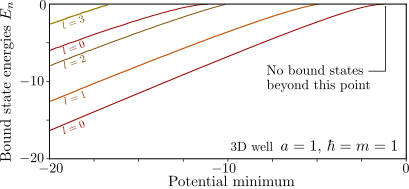
\includegraphics[width=0.65\textwidth]{boundstate3d}
\end{figure}

\section{Quasi-bound states and resonances}

In the 1D finite square well model, there is a sharp distinction
between bound states and free states.  In certain other models,
however, there exist an interesting class of quantum states called
\textbf{quasi-bound states}.  Like a bound state, a quasi-bound state
is localized in one region of space, rather than extending over all
space.  However, it is an \textit{approximate} eigenstate of the
Hamiltonian, and lies within the energy range of the free state
continuum.  As we shall see, the existence of quasi-bound states has
extremely important implications for scattering experiments.

The figure below shows an example of a potential function that can
give rise to quasi-bound states.  In the exterior region, $|x| > b$,
the potential is zero.  Between $x = -b$ and $x = b$, there is a
``barrier'' of positive potential $V_1$.  Embedded in the middle of
this barrier, in the region $|x| < a$, is a central well of depth $U$
such that $0 < V_1 - U < V_1$.

\begin{figure}[h]
  \centering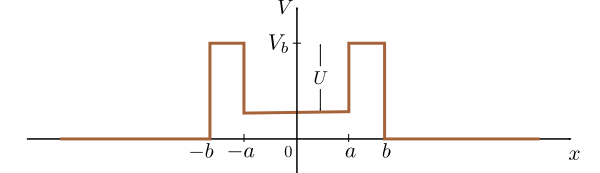
\includegraphics[width=0.7\textwidth]{resonancewell}
\end{figure}

This potential is purely repulsive, so there are no bound states.  The
only exact eigenstates of the Hamiltonian are free states.

However, there's something intriguing about the energy range
corresponding to the central well, $V_1-U < E < V_1$.  Consider a
slightly different situation, where the potential in the exterior
region is $V_1$ rather than $0$; i.e., the potential function is a
finite square well:
$$V_{\mathrm{alt}}(x) = \begin{cases}V_1 - U, & |x| < a, \\ V_1, & \mathrm{otherwise}.\end{cases}$$
In this case, there will be bound states somewhere in the energy range
$V_1-U < E < V_1$.  These bound states' wavefunctions diminish
exponentially away from the square well, and are thus close to zero
for $|x| > b$.  But since $V(x)$ and $V_{\mathrm{alt}}(x)$ differ from
each other only in the region $|x| > b$, these wavefunctions ought to
act as \textit{approximate} solutions to the Schr\"odinger wave
equation for the original potential function $V(x)$---which does not
support bound states!

To understand the implications of these quasi-bound states, let us
analyze the system using the \textbf{scattering experiment} framework
from the previous chapter.  Let a particle be incident from the left,
with energy $E > 0$, described by the incident wavefunction
$$\psi_i(x) = \Psi_i \, e^{ik_i x}.$$
This gives rise to a scattered wavefunction $\psi_s(x)$, such that the
total wavefunction $\psi_i(x) + \psi_s(x)$ satisfies the Schr\"odinger
wave equation with energy $E$.  The scattered wavefunction must be
outgoing (see the previous chapter), so in the exterior region it
takes the form
$$\psi_s(x) = \Psi_i \times \begin{cases}f_- \,e^{-ik_ix}, & x \le -b \\ f_+ \,e^{ik_ix}, & x \ge b.\end{cases}$$
The scattering amplitudes $f_+$ and $f_-$ can be found by solving the
Schr\"odinger wave equation, using the transfer matrix method (see
Appendix B).  The figure below shows numerical results obtained for
$U = 20,\,V_1 = 30,\,a=1$, and $b = 1.2$ or $b = 1.4$, with $\hbar =
m = 1$.

\begin{figure}[h]
  \centering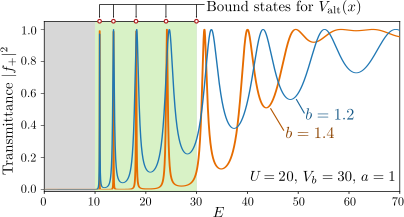
\includegraphics[width=0.65\textwidth]{resonances}
\end{figure}

The vertical axis shows $|f_+|^2$, which is called the
``transmittance'' and measures the probability for the incident
particle to pass through the potential.  The horizontal axis is the
particle energy $E$.  For $E < V_1-U$, the transmittance approaches
zero, and for $E \gtrsim V_1$, the transmittance approaches unity, as
expected.  Within the energy range $V_1-U < E \lesssim V_1$, the
transmittance forms a series of narrow peaks, which get sharper for
larger $b$ (i.e., when the central well is more isolated from the
exterior space).  At the top of the figure, we have also plotted the
bound state energies for the square well potential
$V_{\mathrm{alt}}(x)$, which closely matches the energies of the
transmittance peaks (at least, the first four peaks).

Upon examining the total wavefunction $\psi(x)$ at these special
energies, we see something very interesting.  The figure below plots
$|\psi(x)|^2$ versus $x$ at the energies corresponding to the first
three transmittance peaks, along with the bound state wavefunctions
for the corresponding square well.  We find that $|\psi(x)|^2$ is much
larger within the potential region than the exterior region.
Moreover, its profile is very similar to the corresponding square well
bound state.

\begin{figure}[h]
  \centering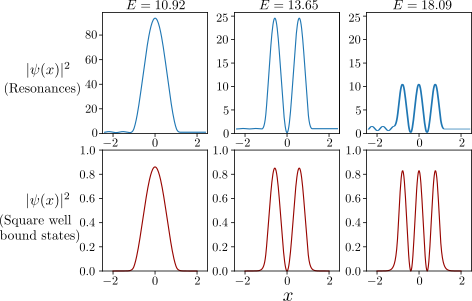
\includegraphics[width=0.75\textwidth]{resonancewavefunctions}
\end{figure}

The enhancement of $|\psi(x)|^2$ is called a \textbf{resonance}.  It
happens because of the existence of a quasi-bound state---an
approximate energy eigenstate that is localized within the scattering
region.  When an incident particle enters the scattering region with
the right energy, it gets temporarily ``trapped'' in the quasi-bound
state, and spends a long time oscillating inside the scatterer before
eventually escaping back to infinity.

This phenomenon is closely analogous to resonances occurring in
classical mechanics, which occur when we take a classical damped
harmonic oscillator and apply an oscillatory driving force.  When the
frequency of the driving force matches the natural frequency of the
oscillator, the system will oscillate with an extremely large
amplitude.  In the quantum mechanical context, the incident
wavefunction plays the role of a driving force, the incident particle
energy plays the role of the driving frequency, and the energy of each
quasi-bound state is like a natural frequency of oscillation.

Resonances play a critical role throughout experimental physics.
Experiments are often conducted for the express purpose of locating
and studying resonances.  When a resonance-induced scattering peak is
found, the location and shape of the peak can be used to deduce
various features of the quasi-bound state, which often provides a
great deal of information about the system itself.

\section{Green's function analysis of scattering resonances}

Quasi-bound states and resonances are not limited to 1D; they are
equally important, if not more so, in 2D and 3D systems.  The Green's
function, introduced in the previous chapter, gives us a very general
tool for studying their properties and consequences.

Let $\hat{H} = \hat{T} + \hat{V}$ be the Hamiltonian of a system
supporting resonances, where $\hat{T}$ is the kinetic energy operator
and $\hat{V}$ is the potential operator.  We decompose the potential
into
$$\hat{V} = \hat{V}_0 + \hat{V}_1,$$
where $V_0$ describes a potential well and $V_1$ describes a potential
barrier.  An example of this decomposition is shown below, for the
1D potential function studied in the previous section.

\begin{figure}[h]
  \centering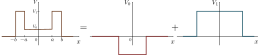
\includegraphics[width=0.99\textwidth]{resonancewell_decomp}
\end{figure}

Let us assume that if the potential consisted of just $\hat{V}_0$
(i.e., the potential well without the barrier), the system has a
single bound state.  Denote this bound state by $|\varphi\rangle$, and
its energy by $E_0$.  Furthermore, let us denote the continuum of free
states for the potential well by $\{|\psi_k\rangle\}$, with energies
$E_k$, where $k$ is some $d$-dimensional continuous index for the free
states.  The bound state and free states satisfy the Schr\"odinger
equation
$$\begin{aligned}\big(\hat{T} + \hat{V}_0\big) |\varphi\rangle &= E_0 |\varphi\rangle \\ \big(\hat{T} + \hat{V}_0\big) |\psi_k\rangle &= E_k |\psi_k\rangle,
\end{aligned}$$
along with the orthogonality and completeness relations
$$\langle\varphi|\psi_k\rangle = 0, \quad |\varphi\rangle\langle\varphi| + \int d^dk\, |\psi_k\rangle\langle\psi_k| = \hat{I}.$$
As described in Section~VII of the previous chapter, the causal
Green's function for this system is
$$\hat{G}_0(E) = \lim_{\varepsilon\rightarrow0^+} \Big(E - \hat{T} - \hat{V}_0 + i\varepsilon\Big)^{-1}.$$

Now, we introduce the barrier potential $\hat{V}_1$.  According to
Dyson's equations (see Section~VI of the previous chapter), the
Green's function for the full problem is
$$\hat{G} = \hat{G}_0 + \hat{G} \hat{V}_1 \hat{G}_0.$$
Our objective is to determine the matrix elements of $\hat{G}(E)$,
which can then be used to compute the scattering amplitudes at each
incident energy $E$.  The eigenstates of the potential well problem,
$|\varphi\rangle$ and $\{|\psi_k\rangle\}$, will be useful for this
purpose.  In particular, note that $|\varphi\rangle$ is not an
eigenstate of $\hat{H}$; it will now play the role of a quasi-bound
state.

As usual when dealing with Dyson's equations, we must watch out for
the fact that $\hat{G}$ appears on both the left and right hand sides.
This can be dealt with by judiciously inserting a resolution of the
identity:
$$\begin{aligned}\hat{G} &= \hat{G}_0 + \hat{G} \hat{I} \hat{V}_1 \hat{G}_0 \\ &= \hat{G}_0 + \hat{G} \left(|\varphi\rangle\langle\varphi| + \int d^dk\, |\psi_k\rangle\langle\psi_k|\right) \hat{V}_1 \hat{G}_0. \end{aligned}$$
We can now compute the matrix element
$\langle\varphi|\cdots|\varphi\rangle$ for both sides of this equation:
$$\begin{aligned}\langle\varphi|\hat{G}|\varphi\rangle = \langle\varphi|\hat{G}_0|\varphi\rangle &+ \langle\varphi|\hat{G}|\varphi\rangle \, \langle\varphi|\hat{V}_1 \hat{G}_0|\varphi\rangle + \int d^dk\, \langle\varphi|\hat{G}|\psi_k\rangle \, \langle\psi_k| \hat{V}_1 \hat{G}_0|\varphi\rangle \\
\langle\varphi|\hat{G}|\varphi\rangle \left(1 - \langle\varphi|\hat{V}_1 \hat{G}_0|\varphi\rangle\right) &= \langle\varphi|\hat{G}_0|\varphi\rangle + \int d^dk\, \langle\varphi|\hat{G}|\psi_k\rangle \, \langle\psi_k| \hat{V}_1 \hat{G}_0|\varphi\rangle \\ \lim_{\varepsilon\rightarrow0^+}
\langle\varphi|\hat{G}|\varphi\rangle \left(1 - \frac{\langle\varphi|\hat{V}_1|\varphi\rangle}{E - E_0 + i\varepsilon}\right) &= \lim_{\varepsilon\rightarrow0^+} \frac{1}{E  - E_0 + i\varepsilon} \left(1+ \int d^dk\, \langle\varphi|\hat{G}|\psi_k\rangle \, \langle\psi_k| \hat{V}_1|\varphi\rangle \right) \\
\lim_{\varepsilon\rightarrow0^+} \langle\varphi|\hat{G}|\varphi\rangle \Big(E - E_0 -\, \langle\varphi|\hat{V}_1|\varphi\rangle \, & + i\varepsilon\Big) - \int d^dk\, \langle\varphi|\hat{G}|\psi_k\rangle \, \langle\psi_k| \hat{V}_1|\varphi\rangle = 1.\end{aligned}$$
Similarly, computing the matrix element
$\langle\varphi|\cdots|\psi_k\rangle$ gives:
$$\begin{aligned}
\langle\varphi|\hat{G}|\psi_k\rangle &= \langle\varphi|\hat{G}_0|\psi_k\rangle + \langle\varphi|\hat{G}|\varphi\rangle \, \langle\varphi|\hat{V}_1 \hat{G}_0|\psi_k\rangle + \int d^dk\, \langle\varphi|\hat{G}|\psi_k\rangle \, \langle\psi_k| \hat{V}_1 \hat{G}_0|\psi_k\rangle \\
&= \lim_{\varepsilon\rightarrow0^+} \left(E-E_k+i\varepsilon\right)^{-1} \left(\langle\varphi|\hat{G}|\varphi\rangle \, \langle\varphi|\hat{V}_1|\psi_k\rangle + \int d^dk\, \langle\varphi|\hat{G}|\psi_k\rangle \, \langle\psi_k| \hat{V}_1|\psi_k\rangle\right)\end{aligned}$$
Note that the equations thus far have been exact (we have \textit{not}
used perturbation theory).  At this point, however, we apply an
approximation: in the last line of the above equation, let the factor
of $\langle\varphi|G|\varphi\rangle$ be large, so that the first term
in the sum becomes dominant over the second term.  It will be shown
below that $\langle\varphi|G|\varphi\rangle$ being large is precisely
the resonance condition, so this approximation will be a
self-consistent one.

With this approximation,
$$\langle\varphi|\hat{G}|\psi_k\rangle \approx \lim_{\varepsilon\rightarrow0^+} \frac{\langle\varphi|\hat{G}|\varphi\rangle \, \langle\varphi|\hat{V}_1|\psi_k\rangle}{E-E_k+i\varepsilon}.$$
Combining this with the other equation gives
$$\lim_{\varepsilon\rightarrow0^+} \left[\langle\varphi|\hat{G}|\varphi\rangle \left(E - E_0 -\, \langle\varphi|\hat{V}_1|\varphi\rangle \, + i\varepsilon\right) - \int d^dk\, \frac{\langle\varphi|\hat{G}|\varphi\rangle\langle\varphi|\hat{V}_1|\psi_k\rangle}{E-E_k+i\varepsilon} \, \langle\psi_k| \hat{V}_1|\varphi\rangle\right] \approx 1.$$
Hence,
$$\boxed{\begin{aligned}\langle\varphi|\,\hat{G}(E)\,|\varphi\rangle \approx \frac{1}{\displaystyle E - E_0 - \langle\varphi|V_1|\varphi\rangle - \Sigma(E)} \qquad \\ \quad \mathrm{where}\;\;\Sigma(E) \equiv \lim_{\varepsilon\rightarrow0^+} \int d^dk\, \frac{\displaystyle| \langle\psi_k| \hat{V}_1|\varphi\rangle|^2}{\displaystyle E-E_k+i\varepsilon}. \qquad
\end{aligned}}$$
The quantity $\Sigma(E)$ is called the \textbf{self-energy}, and we
will have much more to say about it shortly.  It is dependent on $E$,
but let us assume for now that the dependence is weak, so that
$\Sigma$ can be effectively treated as a constant.  It is
complex-valued, and both its real and imaginary parts will be
important.  (We will later show that $\mathrm{Im}(\Sigma) < 0$.)

The above result is extremely meaningful.  It tells us that
$\langle\varphi|\hat{G}(E)|\varphi\rangle$ is large when the
denominator is as close to zero as possible, which is called the
\textbf{resonance condition} (and is self-consistent with the
approximation that we made in the above derivation).  As we vary the
incident energy $E$ over the range of real values, the resonance
condition is satisfied when
$$E \;\approx\; E_{\mathrm{res}} \,\equiv\, E_0 + \langle\varphi|\hat{V}_1|\varphi\rangle + \mathrm{Re}\big[\,\Sigma\,\big].$$
We call $E_{\mathrm{res}}$ the \textbf{resonance energy}.  Its first
term is the energy of the bound state in the absence of the barrier
potential $\hat{V}_1$, and the second term describes the energy shift
induced by $\hat{V}_1$.  The third term is equal to the real part of
the self-energy $\Sigma$, and has a more subtle meaning: since the
definition of $\Sigma$ involves $\{|\psi_k\rangle\}$, we can think of
this term as an energy shift induced by the presence of the continuum
of free states.

In Section VIII of the previous chapter, we derived the following
relationship between the Green's function and the scattering amplitude
$f$:
$$f(\mathbf{k}\rightarrow\mathbf{k}') \;\propto\; \langle \mathbf{k}'|\hat{V}|\mathbf{k}\rangle + \langle \mathbf{k}'|\hat{V}\hat{G}\hat{V}|\mathbf{k}\rangle.$$
Here, $|\mathbf{k}\rangle$ and $|\mathbf{k}'\rangle$ are incident and
scattered plane-wave states satisfying $|\mathbf{k}|=|\mathbf{k}'|$.
The first term describes the lowest-order scattering process (the
first Born approximation).  The second term contains all the
higher-order scattering processes, including resonant scenarios where
the particle bounces around inside the potential before escaping.
By inserting resolutions of the identity between each $\hat{V}$ and
$\hat{G}$ operator in the second term, we find that $f$ contains a
contribution of the form
$$\Delta f(\mathbf{k}\rightarrow\mathbf{k}') \;\propto\; \langle \mathbf{k}'|\hat{V}|\varphi\rangle\langle\varphi|\hat{G}|\varphi\rangle\langle\varphi|\hat{V}|\mathbf{k}\rangle \;=\; \frac{\langle \mathbf{k}'|\hat{V}|\varphi\rangle \, \langle\varphi|\hat{V}|\mathbf{k}\rangle}{\displaystyle E - E_{\mathrm{res}} - i \mathrm{Im}[\,\Sigma\,]}.$$
This can become the dominant contribution to the scattering amplitude
if the resonance condition is satisfied.  The energy dependence of
$\Delta f$ is now determined by its denominator, and has a
characteristic behavior summarized in the figure below:

\begin{center}
  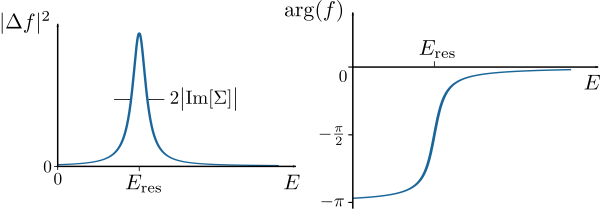
\includegraphics[width=0.7\textwidth]{resonance}  
\end{center}

The graph of $|\Delta f|^2$ versus $E$ has a peaked shape known as a
\textbf{Lorentzian}.  The peak is centered at $E = E_{\mathrm{res}}$,
where the resonance condition is satisfied.  The width of the peak (as
measured by the ``full-width at half-maximum'') is $\delta E \sim
2|\mathrm{Im}[\Sigma]|$.  In other words, the smaller the imaginary
part of the self-energy, the sharper the peak.

The phase, $\mathrm{arg}[\Delta f]$, also contains useful information.
As $E$ crosses $E_{\mathrm{res}}$ from below, the phase increases by
$\pi$.  The energy range over which this phase shift occurs is $\sim
|\mathrm{Im}[\Sigma]|$.

These two resonance signatures---peaks and phase shifts---are sought
after in numerous real-world scattering experiments.  In real
experiments, the peaks and phase shifts are often overlaid on a
``background'' caused by non-resonant effects.  As an example, the
plot below was released by the CMS experiment at the Large Hadron
Collider (LHC), showing a resonance peak on a large background.  This
was part of the experimental evidence that led to the LHC's discovery
of a new particle, the Higgs boson, in 2012.

\begin{figure}[h]
  \centering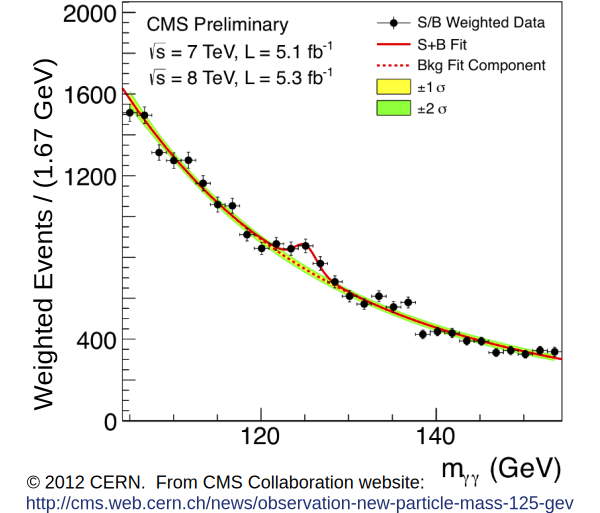
\includegraphics[width=0.45\textwidth]{higgs}
\end{figure}

\section{Fermi's Golden Rule}

We have seen that the width of a resonance is determined by the
imaginary part of the self-energy, $\mathrm{Im}[\Sigma]$.  In this
section, we will show that $\mathrm{Im}[\Sigma]$ has a physical
meaning: it represents the \textbf{decay rate} of a quasi-bound state.
Moreover, it can be approximated using an important formula known as
\textbf{Fermi's Golden Rule}.

Suppose we set the quantum state of a particle to a quasi-bound state
$|\varphi\rangle$ at some initial time $t = 0$.  Because
$|\varphi\rangle$ is not an exact eigenstate of the Hamiltonian, the
particle will not remain in that state under time evolution.  Hence,
for $t > 0$, we expect its wavefunction to become less and less
localized, which can be interpreted as the escape of the particle to
infinity, or as the ``decay'' of the quasi-bound state into the free
state continuum.

The decay process can be described by
$$P(t) = \Big|\langle\varphi|\exp\left(-i\hat{H}t/\hbar\right)|\varphi\rangle\Big|^2,$$
which is the probability for the system to continue occupying state
$|\varphi\rangle$ after time $t$.  In order to calculate $P(t)$, let
us define the function
$$f(t) = \begin{cases} \langle\varphi|\exp\left(-i\hat{H}t/\hbar\right)|\varphi\rangle \,e^{-\varepsilon t}, & t \ge 0 \\ 0, & t < 0,\end{cases}$$
where $\varepsilon \in \mathbb{R}^+$.  For $t \ge 0$ and $\varepsilon
\rightarrow 0^+$, we see that $|f(t)|^2 \rightarrow P(t)$.  The reason
we are interested in $f(t)$, rather than dealing directly with
$\langle\varphi|\exp(-i\hat{H}t/\hbar)|\varphi\rangle$, is that $f(t)$
is more well-behaved.  This function is designed so that firstly, it
vanishes at negative times, prior to start of our thought experiment;
and secondly, it vanishes as $t\rightarrow\infty$ due to the presence
of the ``regulator'' $\varepsilon$.  The latter enforces the idea that
the bound state decays permanently into the continuum of free states,
and can never be re-populated by waves ``bouncing back'' from
infinity.

We can determine $f(t)$ by first studying its Fourier transform,
$$F(\omega) \;=\; \int_{-\infty}^\infty dt \; e^{i\omega t}\, f(t) \;=\; \int_0^\infty dt \; e^{i(\omega + i\varepsilon) t} \; \langle\varphi|e^{-i\hat{H}t/\hbar}|\varphi\rangle.$$
Now insert a resolution of the identity, $\hat{I} = \sum_n
|n\rangle\langle n|$, where $\{|n\rangle\}$ denotes the exact
eigenstates of $\hat{H}$ (for free states, the sum goes to an integral
in the usual way):
$$\begin{aligned}F(\omega) &= \int_0^\infty dt \; e^{i(\omega + i\varepsilon) t} \; \sum_n \langle\varphi|e^{-i\hat{H}t/\hbar}|n\rangle\langle n|\varphi\rangle \\ &= \sum_n \langle\varphi|n\rangle \left( \int_0^\infty dt \; \exp\left[i\left(\omega - \frac{E_n}{\hbar} + i\varepsilon\right) t\right] \right) \langle n|\varphi\rangle \\ &= \sum_n \langle\varphi|n\rangle \frac{i}{\omega - \frac{E_n}{\hbar} + i \varepsilon} \langle n|\varphi\rangle \\ &= i \hbar\; \langle \varphi | \left(\hbar\omega - \hat{H} + i\hbar\varepsilon \right)^{\!-1} | \varphi\rangle. \end{aligned}$$
Note that in the third line, the regulator $\varepsilon$ removes any
contribution from the $t \rightarrow\infty$ limit of the integral (in
accordance with our requirement that the decay of the bound state is
permanent).  Hence,
$$\lim_{\varepsilon \rightarrow 0^+} F(\omega) = i \hbar \, \langle \varphi | \hat{G}(\hbar\omega) | \varphi\rangle,$$
where $\hat{G}$ is our old friend the causal Green's function.  The
appearance of the \textit{causal} Green's function is due to our
definition of the function $f(t)$.

As discussed in the previous section, when the resonance condition is
satisfied,
$$ \langle\varphi|\,\hat{G}(E)\,|\varphi\rangle \approx \frac{1}{\displaystyle E - E_{\mathrm{res}} - i \mathrm{Im}[\Sigma]},$$
where $E_{\mathrm{res}}$ is the resonance energy and $\Sigma$ is the
self-energy of the quasi-bound state.  We can now perform the
inverse Fourier transform
$$\begin{aligned} \lim_{\varepsilon\rightarrow 0^+} f(t) &= \lim_{\varepsilon\rightarrow 0^+} \int_{-\infty}^{\infty} \frac{d\omega}{2\pi} \; e^{-i\omega t} \, F(\omega) \\ &= \frac{i}{2\pi} \int_{-\infty}^{\infty} d\omega\; \frac{e^{-i\omega t}}{\omega - (E_{\mathrm{res}}+i \mathrm{Im}[\Sigma])/\hbar}\\ &= \exp\left(-\frac{iE_{\mathrm{res}}t}{\hbar}\right)\, \exp\left(-\frac{|\mathrm{Im}[\Sigma]|}{\hbar}\,t\right). \end{aligned}$$
In deriving the last line, we performed a contour integration assuming
that $\mathrm{Im}[\Sigma] < 0$; this assumption will be proven
shortly.  The final result is that
$$P(t) = e^{-\kappa t}, \;\;\;\mathrm{where}\;\;\kappa = -\frac{2|\mathrm{Im}[\Sigma]|}{\hbar}.$$
The quantity $\kappa$ describes the rate at which the quasi-bound
state decays away in time.

Let us now take a closer look at the self-energy.  From our earlier
definition,
$$\Sigma(E) \equiv \lim_{\varepsilon\rightarrow0^+} \int d^dk\, \frac{\displaystyle| \langle\psi_k| \hat{V}_1|\varphi\rangle|^2}{\displaystyle E-E_k+i\varepsilon},$$
where $|\varphi\rangle$ and $\{|\psi_k\rangle\}$ are the bound and
free states of the model in the absence of $\hat{V}_1$, and $E_k$ is
the energy of the $k$-th free state.  The imaginary part is
$$\begin{aligned}\mathrm{Im}\big[\Sigma(E)\big] &= \lim_{\varepsilon\rightarrow0^+} \int d^dk\, \Big| \langle\psi_k| \hat{V}_1|\varphi\rangle\Big|^2 \; \mathrm{Im}\left( \frac{1}{\displaystyle E-E_k+i\varepsilon}\right) \\ &= - \int d^dk\, \Big| \langle\psi_k| \hat{V}_1|\varphi\rangle\Big|^2 \; \left[ \lim_{\varepsilon\rightarrow0^+} \; \frac{\varepsilon}{\displaystyle (E-E_k)^2 + \varepsilon^2}\right].\end{aligned}$$
The quantity inside the square brackets is a Lorentzian function,
which is always positive; hence, $\mathrm{Im}(\Sigma) < 0$, as
previously asserted.  The Lorentzian function has the limiting form
$$\lim_{\varepsilon\rightarrow 0^+} \frac{\varepsilon}{x^2+\varepsilon^2} = \pi\delta(x).$$
This comes from the fact that as $\varepsilon\rightarrow0^+$, the
Lorentzian curve describes a sharper and sharper peak, but the area
under the curve is fixed as $\pi$.  Hence,
$$\mathrm{Im}\big[\Sigma(E)\big] = - \pi \int d^dk\, \Big| \langle\psi_k| \hat{V}_1|\varphi\rangle\Big|^2 \; \delta(E-E_k).$$
Because of the delta function, we see that the only non-vanishing
contributions to the integral come from the parts of $k$-space where
$E = E_k$.

We can further simplify the result by defining the \textbf{density of
  states},
$$\mathcal{D}(E) = \int d^d k\; \delta(E - E_k).$$
Roughly speaking, this is a measure of the number of free states with
energy $E$: the $k$-space volume $d^dk$ is proportional to the number
of free states at each given $k$, while the delta function restricts
the contributions to only those free states having energy $E$.  (In
the next section, we'll see an explicit example of how to calculate
$\mathcal{D}(E)$.)  Now, for any function $f(k)$,
$$\int d^d k\; f(k) \, \delta(E - E_k) = \overline{f(k(E))} \;\mathcal{D}(E),$$
where $\overline{f(k(E))}$ denotes the mean value of $f(k)$ for the
free states satisfying $E_k = E$.  Applying this to the imaginary part
of the self-energy gives
$$\mathrm{Im}\big[\Sigma(E)\big] = - \pi \; \overline{\Big| \langle\psi_{k(E)}| \hat{V}_1|\varphi\rangle\Big|^2} \; \mathcal{D}(E).$$
Hence, the quasi-bound state's decay rate is
$$\boxed{\quad\kappa \,=\, -\frac{2}{\hbar}\mathrm{Im}\big[\Sigma(E)\big] \,=\, \frac{2\pi}{\hbar} \; \overline{\Big| \langle\psi_{k(E)}| \hat{V}_1|\varphi\rangle\Big|^2} \; \mathcal{D}(E).\quad}$$
This extremely important result is known as \textbf{Fermi's golden
  rule}.  It says that the decay rate of a quasi-bound mode is
directly proportional to two factors.  The first factor is the mean
squared value of $\langle\psi_{k}| \hat{V}_1|\varphi\rangle$, which is
called the ``transition amplitude'' and describes how $\hat{V}_1$
couples the quasi-bound state and the free states; note that this
factor goes to zero when $\hat{V}_1 = 0$, which is the case where
$|\varphi\rangle$ is a true bound state (which does not decay).  The
second factor is the density of free states available for
$|\varphi\rangle$ to decay into.

\section{Fermi's golden rule in a 1D resonance model}

\begin{figure}[h]
  \centering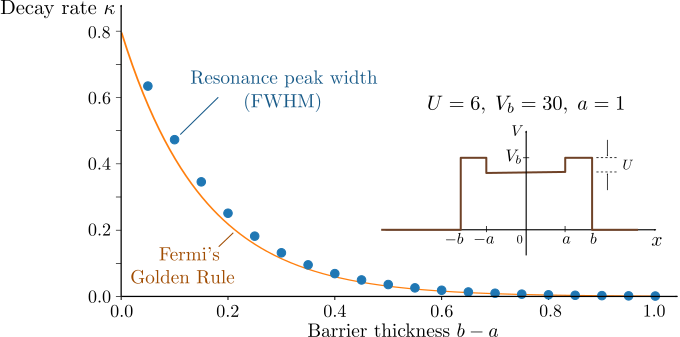
\includegraphics[width=0.85\textwidth]{goldenrule}
\end{figure}

\section*{Exercises}

\begin{enumerate}
\item Existence of bound states in 1D
\label{ex:boundstate}

\item In this problem, you will investigate the existence of bound
  states in a 3D potential well that is finite, uniform, and
  spherically-symmetric.  The potential function is
$$V(r,\theta,\phi) = -U\Theta(a-r),$$
  where $a$ is the radius of the spherical well, $U$ is the depth,
  and $(r,\theta,\phi)$ are spherical coordinates defined in the usual
  way.

  The solution involves a variant of the partial wave analysis
  discussed in Appendix A.  For $E < 0$, the Schr\"odinger equation
  reduces to
$$\begin{cases}\Big(\nabla^2 + q^2\Big) \psi(r,\theta,\phi) = 0 \;\;\mathrm{where}\;\; q = \sqrt{2m(E+U)/\hbar^2}, \;\;&\mathrm{for} \; r \le a \\ \Big(\nabla^2 - \gamma^2\Big) \psi(r,\theta,\phi) = 0 \;\;\mathrm{where}\;\; \gamma = \sqrt{-2mE/\hbar^2}, \;\;&\mathrm{for} \; r \ge a. \end{cases}$$
  For the first equation (called the Helmholtz equation), we seek
  solutions of the form
  $$\psi(r,\theta,\phi) = f(r) \, Y_{\ell m}(\theta,\phi),$$
  where $Y_{\ell m}(\theta,\phi)$ are
  \href{https://en.wikipedia.org/wiki/Spherical_harmonics}{spherical
    harmonics}, and the integers $l$ and $m$ are angular momentum
  quantum numbers satisfying $l \ge 0$ and $-l \le m \le l$.
  Substituting into the Helmholtz equation yields
  $$r^2\frac{d^2f}{dr^2} + 2r \frac{df}{dr}+\left[q^2r^2-l(l+1)\right] f(r) = 0,$$
  which is the \textbf{spherical Bessel equation}.  The solutions to
  this equation that are non-divergent at $r = 0$ are $f(r) =
  j_\ell(qr)$, where $j_\ell$ is called a \textbf{spherical Bessel function
    of the first kind}.  Most numerical packages provide functions to
  calculate these (e.g.,
  \href{https://docs.scipy.org/doc/scipy/reference/generated/scipy.special.spherical_jn.html}{\texttt{scipy.special.spherical\_jn}}
  in Scientific Python).

  Similarly, solutions for the second equation can be written as
  $\psi(r,\theta,\phi) = g(r) \, Y_{\ell m}(\theta,\phi),$ yielding an
  equation for $g(r)$ called the \textbf{modified spherical Bessel
    equation}.  The solutions which do not diverge as $r\rightarrow
  \infty$ are $g(r) = k_\ell(\gamma r)$, where $k_\ell$ is called a
  \textbf{modified spherical Bessel function of the second kind}.
  Again, this can be computed numerically (e.g., using
  \href{https://docs.scipy.org/doc/scipy/reference/generated/scipy.special.spherical_kn.html#scipy.special.spherical_kn}{\texttt{scipy.special.spherical\_kn}}
  in Scientific Python).

  Using the above facts, show that the condition for a bound state to
  exist is
  $$\frac{qj_\ell'(qa)}{j_\ell(qa)} = \frac{\gamma k_\ell'(\gamma a)}{k_\ell(\gamma a)},$$
  where $j_\ell'$ and $k_\ell'$ denote the derivatives of the relevant
  special functions, and $q$ and $\gamma$ depend on $E$ and $U$ as
  described above.  Write a program to search for the bound state
  energies at any given $a$ and $U$, and hence determine the
  conditions under which the potential does not support bound
  states.



\label{ex:boundstate3d}

\item Phase shift under scattering resonance

\item Classical driven oscillator analogy  
\end{enumerate}




\section*{Further Reading}

\begin{itemize}
\item Bransden \& Joachain, \S4.4, 9.2--9.3, 13.4
\item Sakurai, \S5.6, 7.7--7.8

%% \item 
%%   C.~W.~Hsu, B.~Zhen, A.~D.~Stone, J.~D.~Joannopoulos, and
%%   M.~Solja\u{c}i\'{c}, \textit{Bound states in the continuum},
%%   Nature Reviews Materials \textbf{1}, 16048 (2016).
%%   \label{cite:hsu}
\end{itemize}

\end{document}


%% For decades after the discovery of quantum mechanics, the quantum
%% double-slit experiment was just a ``thought experiment'', meant to
%% illustrate the features of quantum mechanics that had been uncovered
%% by other, more complicated experiments.  Nowadays, the most convenient
%% way to do the experiment is with light, using single-photon sources
%% and single-photon detectors.  Quantum interference has also been
%% demonstrated experimentally using electrons, neutrons, and even
%% large-scale particles such as buckyballs.
